%
%  This is an example LaTeX file. The percent sign is used to mark the
% start of a comment.
%
%  - Michael Weeks, January, 2003
%
\documentclass[conference]{IEEEconf}
\usepackage[dvips]{graphics}
\usepackage{tikz}
\usepackage{dtklogos}
\usepackage[utf8]{inputenc}
\usetikzlibrary{mindmap}
\usepackage[hidelinks,pdfencoding=auto]{hyperref}
\usepackage{dirtree}
% Information boxes
\newcommand*{\info}[4][16.3]{%
  \node [ annotation, #3, scale=0.65, text width = #1em,
          inner sep = 2mm ] at (#2) {%
  \list{$\bullet$}{\topsep=0pt\itemsep=0pt\parsep=0pt
    \parskip=0pt\labelwidth=8pt\leftmargin=8pt
    \itemindent=0pt\labelsep=2pt}%
    #4
  \endlist
  };
}


\IEEEoverridecommandlockouts % Don't forget this command!

\begin{document}
  \title{Data Driven Approach For Transfer Data  From ANT+ Sensors}

  \author{{Petr Je\v{z}ek$^{1}$, Roman Mou\v{c}ek$^{1}$}
\thanks{$^{1}$Department of Computer Science and Engineering
New Technologies for the Information Society
Faculty of Applied Sciences
University of West Bohemia
Plzen, Czech Republic
        {\tt\small {jezekp, moucek}@kiv.zcu.cz}}%
\thanks{*Acknowledgements will be added}% <-this % stops a space
}
\maketitle


\begin{abstract}
This is the abstract. You can use this file to start your own LaTeX file,
and just delete the stuff you do not need. \LaTeX  is a lot like working
with HTML: you can specify where text effects begin, and where they end.This is the abstract. You can use this file to start your own LaTeX file,
and just delete the stuff you do not need. \LaTeX  is a lot like working
with HTML: you can specify where text effects begin, and where they end.This is the abstract. You can use this file to start your own LaTeX file,
and just delete the stuff you do not need. \LaTeX  is a lot like working
with HTML: you can specify where text effects begin, and where they end.This is the abstract. You can use this file to start your own LaTeX file,
and just delete the stuff you do not need. \LaTeX  is a lot like working
with HTML: you can specify where text effects begin, and where they end.
\end{abstract}

\section{Introduction}\label{sec:intro}
Managing diseases and health issues is worldwide still more expensive especially with aging population. For instance there are around 23 million people affected with heart failure \cite{bui2011epidemiology}. These people have been treated in hospitals for a long time. Nowadays, the situation is changing because relatively cheap solutions for a home treatment is coming to the market \cite{4761985, 5333913}. These solutions enable to make a particular shift of patients from hospitals to their homes. It brings advantages in better comfort for patients and cheapens treatment itself. These solutions usually use a set of sensors for monitoring of a health level. Wearable sensors are usually powered from batteries. They have to operate for a long time period without possibility to change batteries frequently. As a solution new protocols with the objective of low energy consumption as ZigBee \cite{Farahani:2008:ZWN:1457417}, Bluetooth Low Energy \cite{heydon2012bluetooth} or ANT \cite{zaloker2014ant} has been defined.  Data from these sensors are transfered to remote servers where they are processed and results are visualized to the user. Sensors usually measure a large collection of body parameters. Integration of these sensors creates a Body Area Networks (BAN). When the number of sensors connected to BAN is increasing a management and a long term storage and sustainability of data is a major requirement in future applications.

While low energy consumption standards for data transfer exist they are still too fragmented to enable an easy manipulation with obtained data. As a solution this paper presents an approach of using a unified HDF5 format for encapsulating ANT+ sensor data and its transfer to a remote storage. 

The paper is organized as follows. Section \ref{sec:state-of-the-art} describes current approaches in the domain then Section \ref{sec:ant-plus-profiles} describes existing ANT+ profiles and selects most suitable profiles for eHealth domain. Section \ref{sec:framework} describes proposed framework that facilitates the conversion of sensors data to an output HDF5 format. Then Section \ref{sec:use-case} demonstrates the usage of proposed transformation. Last Section \ref{sec:future-work} summarizes the current work and provide an outlook to the future.

\section{State of The Art}\label{sec:state-of-the-art}

An approach presented in \cite{mehmood2014ontology} defines a three layers ontology describing data from different sensors. This ontology can facilitates programmer development of tools for processing sensors data. A Sensor-Cloud infrastructure \cite{5635688} represents physical sensors as virtual sensors stored in a Cloud infrastructure. The Cloud manages sensors capability. So called Semantic Sensor Web \cite{4557983} is based on an annotation of sensors data by means of Semantic Web. Such annotated data can be distributed via the Internet.


\section{ANT+ Profiles Discussion}\label{sec:ant-plus-profiles}
ANT+ protocol is popular because of its low energy consumption and because it provide good means to describe body parameters or fitness level. The main benefit are ``device profiles`` to define how to send data over the network in a consistent way \cite{innovations2013ant}. When the data transfer profiles are defined they facilitates development of sensors. 
ANT+ profiles supports a large scale of activities such as Cycling, Walking or devices for measurement of Heart Rate, Blood pressure, Weight, Muscle Oxygen Monitor etc. If we browse individual profiles detailed we can observe attributes that are common for all profiles including e.g.: device name, status, manufacturer, signal strength or battery status. Then, there are other attributes varying for individual profiles. 

According to individual attributes we can define common attributes as metadata of sensors while individual profile attributes represent raw sensor data. 

\section{Proposed Framework}\label{sec:framework}

\subsection{Requirements}\label{sec:requirements}

Due to the absence of a format or a data structure for representing data coming from sensors we are designing a framework that enables collecting of sensor data and storing both raw data and metadata. The framework have to use a widely accepted format in order to stored data can be reused in third-party systems.

\begin{figure*}
\centering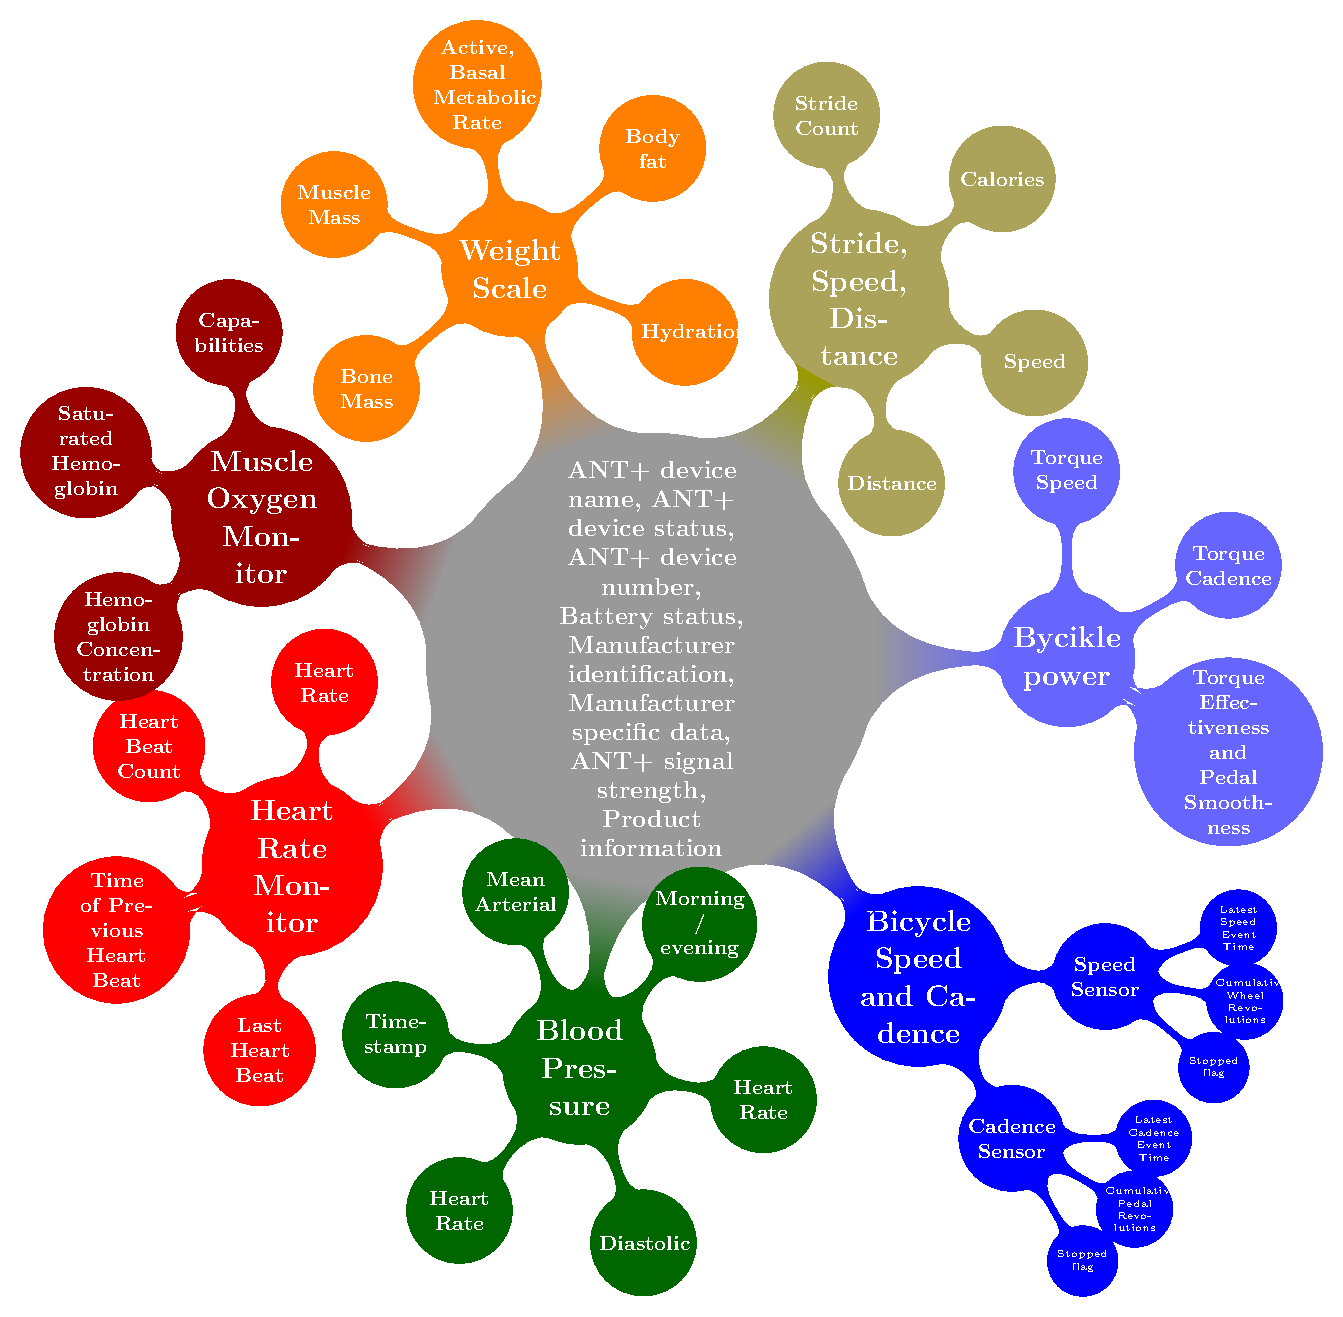
\includegraphics[width=12cm, height=10cm]{AntPlusProfiles}
\caption{\label{AntPlus}ANT+ Profiles Network}
\end{figure*}

\subsection{Format Discussion}

In Section \ref{sec:ant-plus-profiles} ANT+ data has been defined as a combination of raw data supplemented by descriptive metadata. Therefore the developed format has to be robust to enable handling with large collections of raw data and simultaneously must be flexible to deal with heterogeneous metadata.

As a member of International Neuroinformatics Coordinating Facility (INCF) \cite{wvangeit:Bjaalie:JNeurosci:2007} we are responsible for development of hardware and software infrastructure for electrophysiology experiments. Within INCF we are a member of the working group of the INCF Task Force on Electrophysiology\footnote{http://www.incf.org/programs/datasharing/ electrophysiology-task-force}. There were introduced two approaches towards defining a standard. The first one uses the Hierarchical Data Format (HDF5) \cite{hdf5}. HDF5 is portable and extensible format supporting an unlimited variety of datatypes and is designed for flexible and efficient I/O and for high volume and complex data. The second approach is OdML~\cite{10.3389/fninf.2011.00016}. It is a~free form tree-like structure of sections, properties and values. It is a suitable metadata format because of its platform-independence, simplicity, and human-readability. Moreover, it ensures a compatibility with other systems developed in neuroinformatics community, for example \cite{10.3389/conf.fninf.2014.18.00029}, \cite{10.3389/conf.fninf.2014.18.00053}, and~\cite{10.3389/conf.fninf.2013.09.00025}. A next step is merging of these two approaches\cite{10.3389/conf.fninf.2013.09.00069}. The NIX format~\cite{Stoewer:2014} provides a data model for storing experimental data in HDF5, together with metadata in the odML format.




\subsection{Proposed Mapping}

We selected these ANT+ profiles that can be used for monitoring of person health or fitness level. We selected a common metadata from these profiles and individual raw data. Figure \ref{AntPlus} show a graphical relationship of the profiles. A middle gray circle shows common metadata while other circles are selected profiles and their raw data. 


The NIX model for data consists of several main elements: Block, DataArray, Tag, MultiTag, Source, Group and Dimension. Each element consists several attributes such as id, name and specific attributes for individual elements. Moreover, each elements can consist a link to an odML metadata model. We use a simplified model for mapping ANT+ elements. A Source represents an ANT+ device, the DataArray represents raw data coming from the device sensor, the Dimension represents a description of axis. Last, the Block wraps complete recording.

\section{Use Case}\label{sec:use-case}

The presented framework serves mainly for designers or programmers of complete systems intended for home monitoring of end-users. We suppose that such a programmer want to implement a system for heart rate monitoring of elderly people. This system have following requirements: It must use a easy to use sensor for a heart rate monitoring, data from this sensor must be easily transferred to a computer where they are stored and eventually evaluated. Moreover there are regular medical checks where a physician can use these long term heart rate records to check a health condition of the patient or eventually set a treatment. This requires to both the patient and the doctor use software with readable format. 

As a solution so called neuroinformatics databases and approaches such as CRCNS \cite{CRCNS}, Helmholtz \cite{10.3389/conf.fninf.2013.09.00025}, Carmen \cite{fgibson:Watson2007},  INCF Dataspace \cite{dataspace} or EEGBase \cite{ISI:000306821100004} are developing. These databases are the most promising approaches they could accept NIX format as a standardized one.

There is lot of heart rate monitor straps. We use Garmin Premium Strap Heart Rate Monitor for this use-case. It is an ANT+ supported device, we use Android SDK\footnote{http://developer.android.com/sdk/} that enable reading data by Android smart phones. We integrate the SDK into a custom mobile application MoBio\footnote{https://github.com/NEUROINFORMATICS-GROUP-FAV-KIV-ZCU/MoBio} that reads data from ANT+ sensors and store them on a SD card. The user can pair available sensors, record data and visualize them. This solution can be accepted by large scale of users because of cheap Android smart phones and heart rate monitor straps on the market.

Finally, MoBio integrates our framework we can store data into a NIX file. When MoBio reads data it parses basic metadata such as device name, product information etc. We transfer them into structure with a one section and several properties as it is expressed in Figure \ref{odML}. Then heart beats are continuously read. We store these beats into a data array. Figure \ref{NIX-ex} shows a signal stored in a DataArray. A Source has an attribute metadata that contains a link to metadata stored in the odML structure.

Once data are stored they can be transferred to a suitable neuroinformatics database. Figure \ref{fig:EEGBase} shows data stored in EEGBase. There is a complex description of an experiment containing also metadata from Heart Rate strap. The raw data are stored as well.

\begin{figure}

\dirtree{%
.1 Section.
.2 name = heart\_rate.
.2 type = metadata.
.2 Properties.
.3 Device name = Strap heart rate monitor.
.3 Device number = 1.
.3 Product Information = Garmin Premium Strap Heart Rate Monitor.
}
\caption{\label{odML}odML metadata for heart rate sensor}
\end{figure}

\begin{figure*}
\centering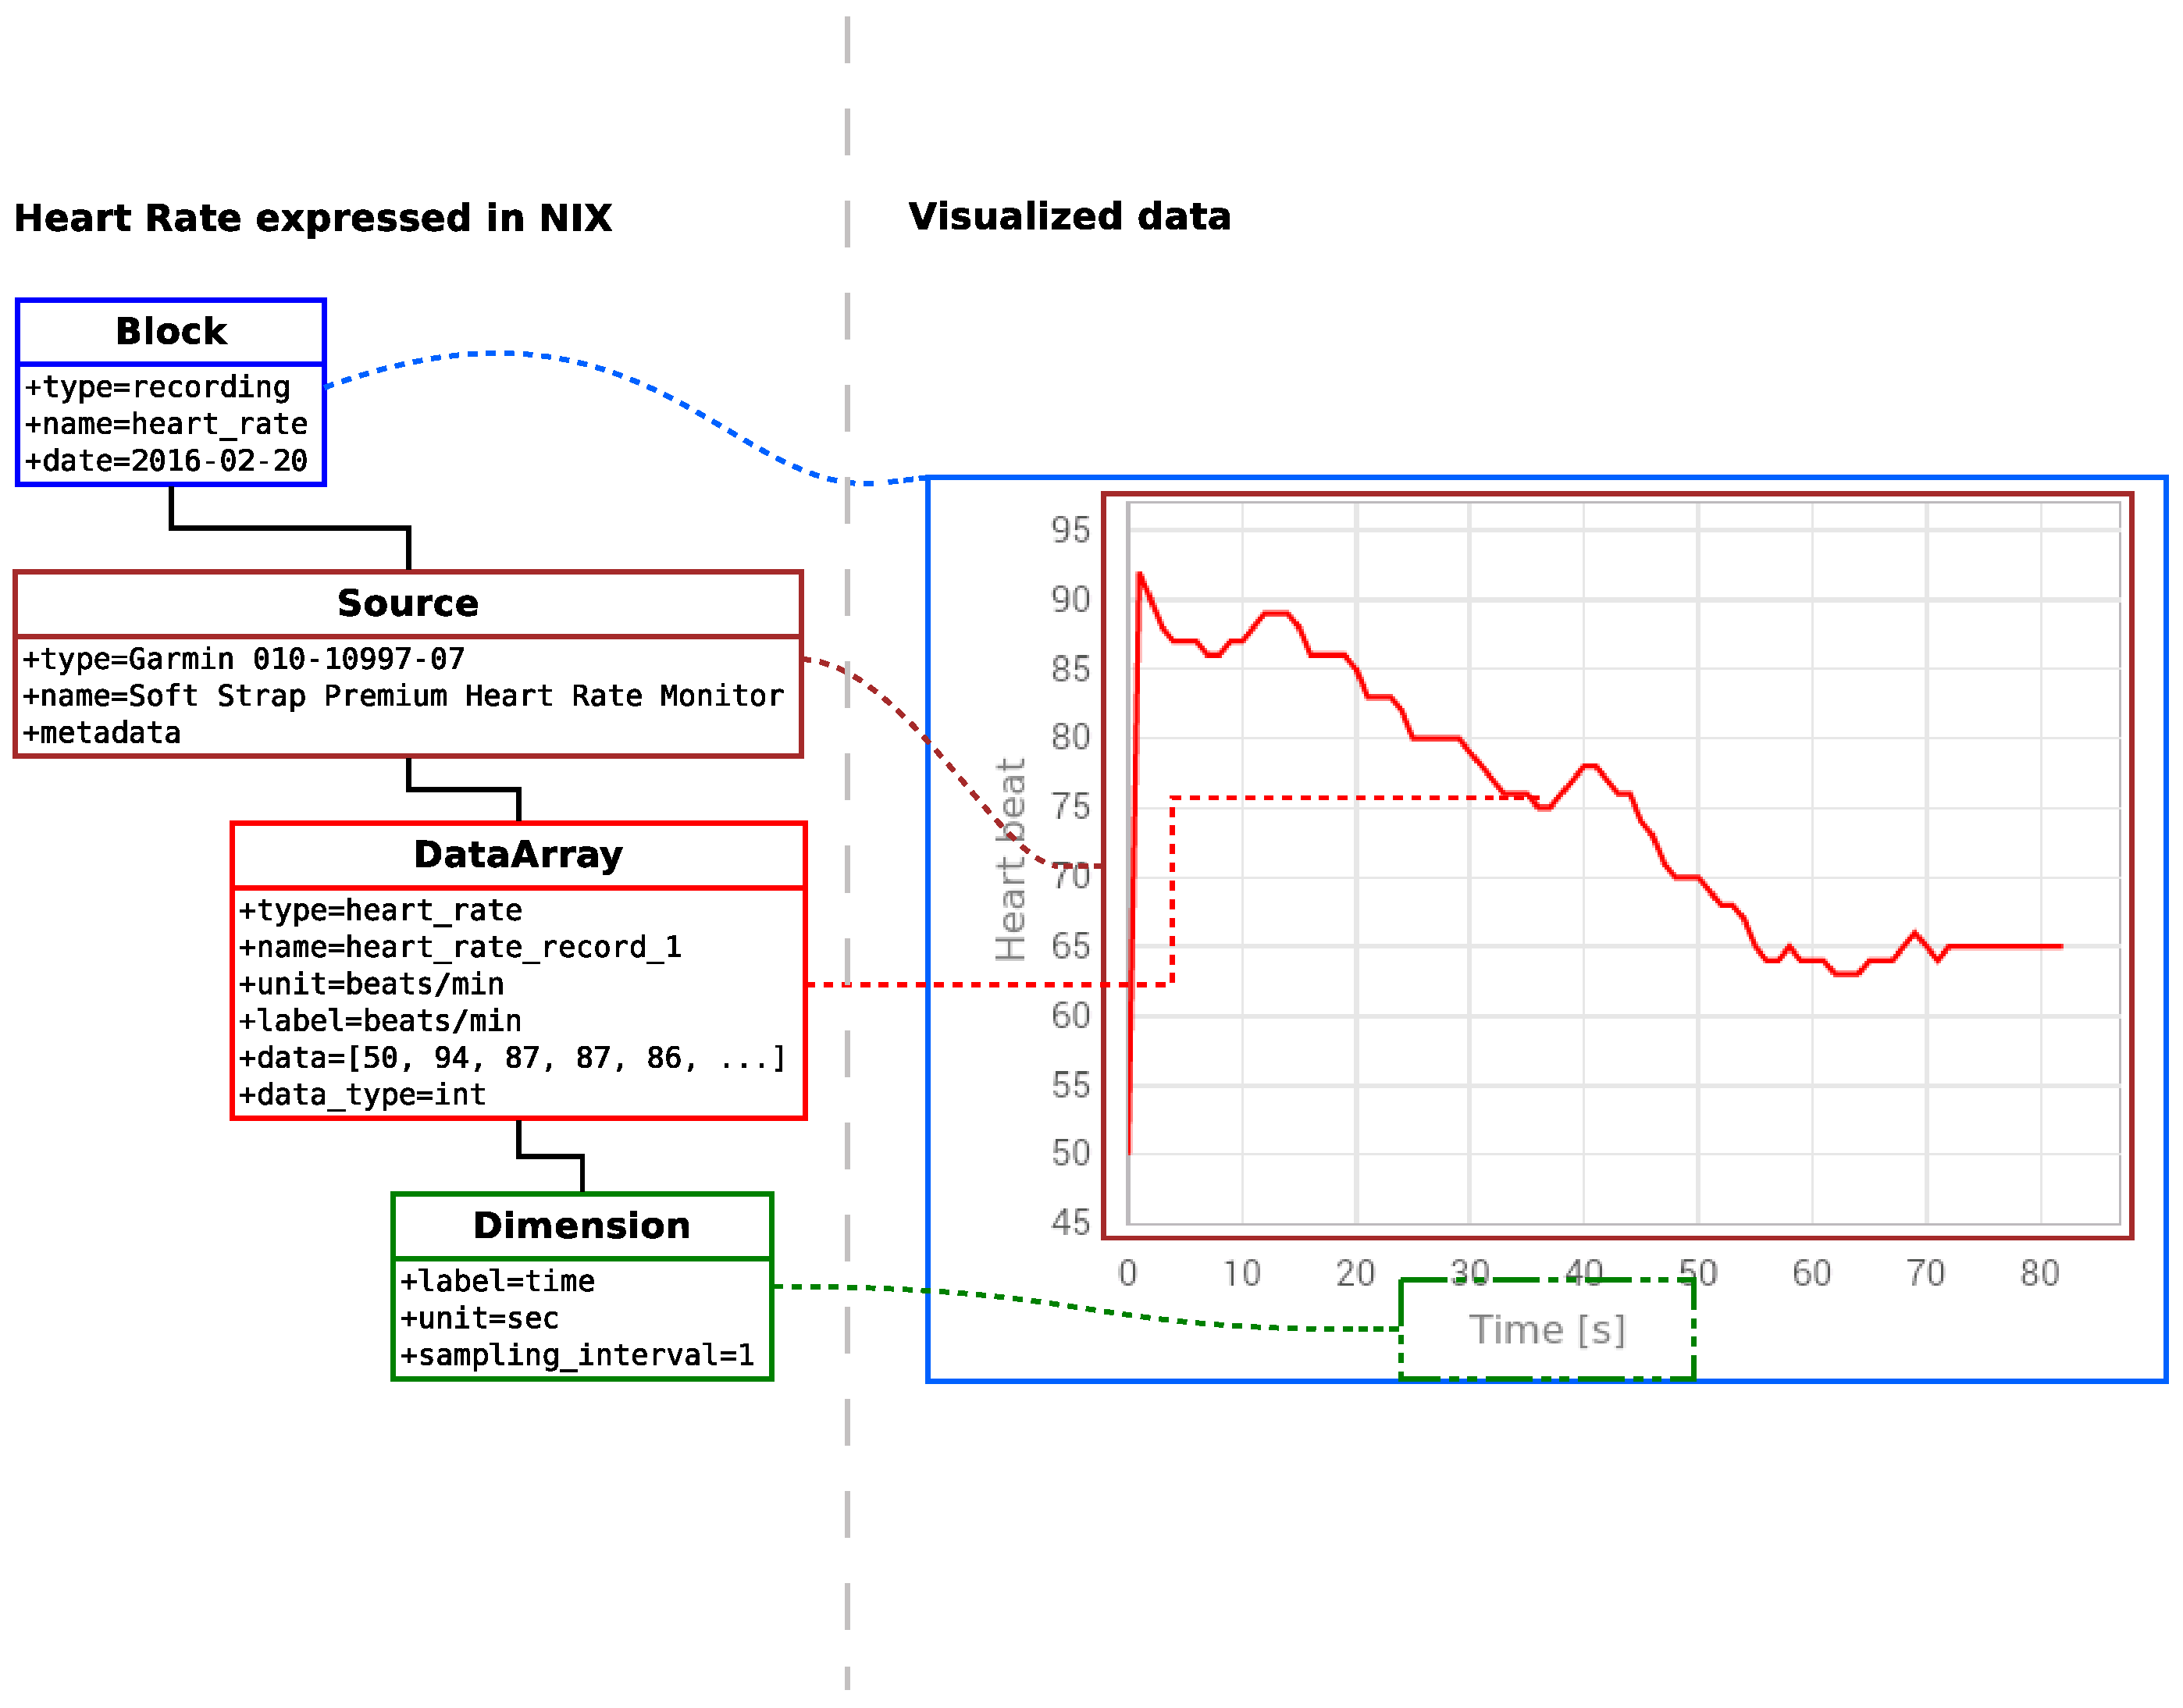
\includegraphics[width=13cm]{NIX-example}
\caption{\label{NIX-ex}Heart rate measurement transferred to NIX}
\end{figure*}

\begin{figure}
  %\vspace{-0.2cm}
  \centering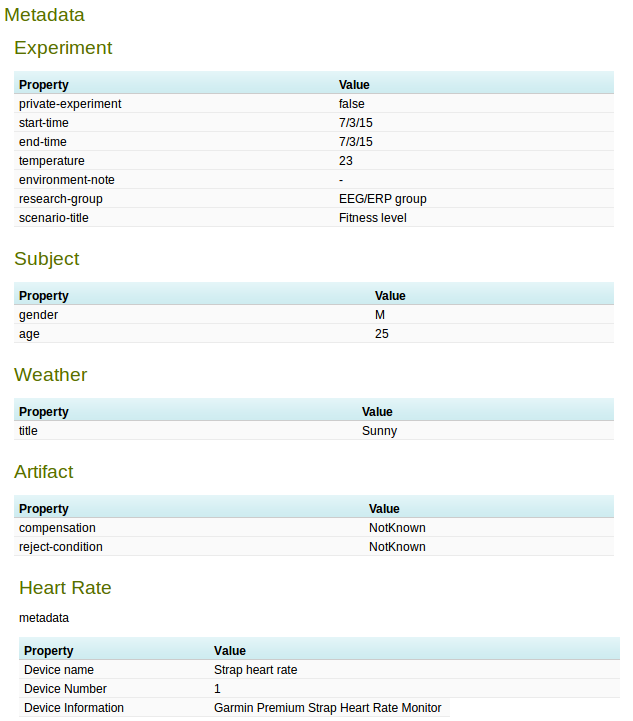
\includegraphics[width=8cm]{portal_example.png}
  \caption{Data stored in EEGBase}
  \label{fig:EEGBase}
 \end{figure}


\section{Conclusions and Future Work}\label{sec:future-work}





% Now here is the reference section.

\bibliographystyle{IEEEtran}
% argument is your BibTeX string definitions and bibliography database(s)
\bibliography{EMBC-2016,citations-ic4awe-2016,bibliography,neuroportals}
\end{document}